\documentclass[conference]{IEEEtran}
\IEEEoverridecommandlockouts
% The preceding line is only needed to identify funding in the first footnote. If that is unneeded, please comment it out.
\usepackage{cite}
\usepackage{amsmath,amssymb,amsfonts}
\usepackage{algorithmic}
\usepackage{graphicx}
\usepackage{textcomp}
\usepackage{hyperref}
\usepackage{xcolor}
\usepackage{listings}
\usepackage{enumitem}
\usepackage{todonotes}
\usepackage{subcaption}
\usepackage{fancyhdr}
\usepackage{float}

\lstdefinestyle{javastyle}{
    basicstyle=\ttfamily\footnotesize,
    breakatwhitespace=false,         
    breaklines=true,                 
    captionpos=b,                    
    keepspaces=true,                 
    numbers=left,                    
    numbersep=5pt,                  
    showspaces=false,                
    showstringspaces=false,
    showtabs=false,                  
    tabsize=2,
    language=Java,
    frame=single,
}

\lstset{style=javastyle}

\def\BibTeX{{\rm B\kern-.05em{\sc i\kern-.025em b}\kern-.08em
    T\kern-.1667em\lower.7ex\hbox{E}\kern-.125emX}}
\begin{document}

\title{Trace-Based Bytecode Interpreter Visualization for Compiler Construction Education \\ Artifact Description}

\author{\IEEEauthorblockN{\href{https://orcid.org/0000-0003-0771-2257}{Tobias Herber}}
\IEEEauthorblockA{\emph{Institute for System Software} \\
\emph{Johannes Kepler University}\\
Linz, Austria \\
tobias@herber.space
}
\and
\IEEEauthorblockN{\href{https://orcid.org/0000-0002-8232-5030}{Markus Weninger}}
\IEEEauthorblockA{\emph{Institute for System Software} \\
\emph{Johannes Kepler University}\\
Linz, Austria \\
markus.weninger@jku.at
}
}

\maketitle

% Author version information
\fancypagestyle{firstpage}{%
\fancyhead{}
\renewcommand\headrule{}
\fancyfoot[C]{\small
This document is an extension of ``\emph{Trace-Based Bytecode Interpreter Visualization for Compiler Construction Education}'' by Herber and Weninger, describing the artifacts of said work~\cite{herber2025}. A video accompanying this artifact can also be found at \url{https://ssw.jku.at/General/Staff/Weninger/Projects/InterpreterViz/VISSOFT25/Video.mp4}.}
}
\thispagestyle{firstpage}

\begin{abstract}

% Understanding compiler construction and bytecode interpretation is a challenging task for students due to the abstract nature of these concepts.
Enhancing students' comprehension of bytecode generation and its interpretation is crucial, yet challenging, in compiler construction courses. 
Traditional approaches often emphasize theoretical concepts, making it difficult for students to grasp the inner workings of bytecode interpreters.

To bridge this gap, we introduce a web-based tool for \emph{trace-based bytecode interpreter visualization}, designed to enhance comprehension by providing an interactive and visually enriched learning experience. 
%Our tool provides a view that aligns bytecode operations with high-level source code.
%Besides that, dynamic and interactive visualizations illustrate changes in memory, register states, and control flow through animations, symbol annotations, and call/jump indicators.
%Moreover, we utilize symbol information, e.g., variable names, to support users in easier seeing relations.
Our tool provides a side-by-side view that aligns the original high-level source code and its corresponding low-level bytecode, with arrows indicating jumps and method calls.
Users can step through the executed bytecode (forwards and backwards) to see the effect of each operation.
A dynamic memory visualization utilizes animations to illustrate changes in the interpreter's various memory regions and its registers.
To further increase the flexibility of our tool, we developed a lightweight metalanguage that enables educators to define visualizations for arbitrary bytecode formats.
% Symbol information, e.g., variable names, are used to simplify all our visualizations. % optional

Our tool aims to bridge the gap between abstract theory and concrete execution.
We demonstrate its effectiveness in various educational settings, e.g., how it can help educators improve their live teaching and how it facilitates student self-study.

%Extensibility is a key feature of our system.
% To make our tool suitable for a wide range of scenarios

% We detail the design and implementation of our tool, outlining the architectural choices, meta-language structure, and technical concepts used by our tool.

\end{abstract}

\begin{IEEEkeywords}
Compiler Construction, Bytecode Interpreter, Visualization, Interactive Learning, Debugging, Trace-Based Debugging, Computer Science Education
\end{IEEEkeywords}

\section{Introduction}

This document accompanies the paper ``\emph{Trace-Based Bytecode Interpreter Visualization for Compiler Construction Education}'', by Herber and Weninger, and serves as a supplement describing the artifacts developed as part of the work~\cite{herber2025}. It provides a technical overview of the visualization tool introduced in the paper, along with concrete examples and demonstration files that showcase its functionality in practice.

While the main paper focuses on the conceptual design, motivation, and educational applications of our visualization approach, this artifact description centers on the practical implementation.

The document is organized into the following key sections:

\begin{itemize}
    \item an introduction of our main feature set,
    \item a brief overview of the technical implementation as well as the structure of or code base,
    % \item an overview of our trace format as well as our domain-specific language (DSL) for visualization specification,
    \item a walkthrough of 5 concrete bytecode traces demonstrating the features of our visualization tool.
\end{itemize}

Where applicable, references to relevant sections of the paper are provided to connect the described features to their theoretical foundations.

\section{Included Artifacts}

% Wir müssten also des microjava projekt nicht dabei haben:
% Complete: To the extent possible, all components relevant to the paper in question are included. (Proprietary artifacts need not be included. If they are required to exercise the package, then this should be documented, along with instructions on how to obtain them. Proxies for proprietary data should be included so as to demonstrate the analysis.)

Our artifact includes the main web-based visualization tool (located in \texttt{visualizer.zip}) as well as a set of demonstration bytecode traces (located in \texttt{demos.zip}). These bytecode traces have been generated using a modified version of the \emph{MicroJava} VM (see \cite{herber2025}, Section II-C). The demo traces should serve as a good testing ground for our project.
More details on MicroJava (not needed to exercise this artifact) are given in~\cite{moessenboeck2025compiler} and a reference compiler and VM for MicroJava can be found at~\cite{moessenboeckWeb}.

\section{Tool Functionality}

The functionality of our visualization tool is described in detail in our main publication. This section outlines the core functionality that will serve as the basis for this technical overview.

\begin{itemize}
    \item \emph{Interactive Execution Playback}: Users can step through the execution trace of a program's bytecode both forward and backward. This enables detailed inspection of the interpretation of a program at each operation, supporting fine-grained program analysis, and enhancing comprehension (see \cite{herber2025}, Section IV).

    \item \emph{Jump and Playback Controls}: Users can jump directly to specific bytecode or source code positions, or use a slider and control buttons to navigate through the execution. An optional “play until” feature animates execution until a selected target is reached.

    \item \emph{Combined Code Visualization}: The tool displays the original high-level source code along with its compiled bytecode. It dynamically highlights the current position in the source code and bytecode. Our tool supports special visualizations for control flow, such as arrows indicating the destinations of jump operations (see \cite{herber2025}, Section V).

    \item \emph{Animated Memory Visualization}: The interpreter's memory regions (stack, heap, globals, etc.) are shown as distinct animated views. Memory changes (allocations, mutations, arithmetic, control flow) are visualized in real time, with support for displaying symbol information such as variable names and types.

    \item \emph{Execution Trace Format}: The underlying execution trace format is log-structured and allows for easy extension of our visualization to other bytecode formats. It includes a recoding of all executed operations, including, the operation and its operands, updated memory pointers, and additional values, such as the computed results of an arithmetic operation, or the source and destination addresses of a move operation.

    \item \emph{Customizable Visualization via DSL}: A domain-specific language (DSL) defines the semantics of bytecode operations and the structure of memory regions. This allows the tool to support other bytecode formats beyond MicroJava, and provides a clean abstraction layer for extending visualization behavior.

    \item \emph{Reference Bytecodes}: The tool highlights mismatches between actual and expected bytecode sequences, supporting comparison against reference implementations. This feature can aid students in debugging their own faulty compiler implementations.

    \item \emph{Interpreter Error Reporting}: Runtime errors are captured during trace collection and displayed in the visualization, enabling diagnosis of the execution leading up to an interpreter error.

\end{itemize}

These features make the tool a powerful resource for both educators and students in compiler construction and provide an accessible platform for exploring the behavior of bytecode interpreters through interactive, animated execution traces.

\section{Developer Overview}

In this section, we provide an overview of our project's structure as well as select implementation components. Moreover, we describe the steps to start a development version of our visualization tool using the provided artifacts. 

\subsection{Core Implementation Details}

Our visualization is written in Typescript\footnote{Typescript \url{https://www.typescriptlang.org/}}, a statically typed superset of JavaScript, which allows us to perform compile-time type checking on JavaScript code. The user interface (UI) is implemented using the React\footnote{React \url{https://react.dev/}} framework, which allows us to write component-based UIs by writing markup directly in TypeScript (so-called JSX \footnote{JSX in Typescript \url{https://www.typescriptlang.org/docs/handbook/jsx.html}}). While we implemented our own animation orchestration framework, the underlying animations are executed using the Framer Motion\footnote{Framer Motion \url{https://www.npmjs.com/package/framer-motion}} library. The Vite-bundler \footnote{Vite \url{https://vite.dev/}} is used to transform developer-written TypeScript code into highly optimized JavaScript code which browsers can execute natively.

\subsection{File Structure}

The compressed folder \texttt{visualizer.zip} contains our web-based visualization project. This folder contains a \texttt{package.json} file which describes the build and start scripts of our project as well as the dependencies needed to to run it. The \texttt{src} folder contains the TypeScript files used to implement our tool.

The source code is grouped into several modules located in the \texttt{src/modules} folder:

\begin{itemize}
    \item The \texttt{lib} module which includes several utility functions, mostly for manipulating the browser's DOM tree \footnote{DOM \url{https://developer.mozilla.org/en-US/docs/Web/API/Document_Object_Model/Introduction}} as well as functions for managing application state.

    \item The \texttt{memory} module implements our memory snapshot functionality. The state of our visualization is supported by memory snapshots. These memory snapshots are generated by the visualization specification DSL implementation. The developer of a visualization specification can simply manipulate a memory snapshot to define the behavior of each bytecode operation.

    % note to self: for the main thesis we should also include the diffing stuff here

    \item The \texttt{operation-trace} module implements the parser for our trace format. This format is implemented as a log-structure which contains various JSON objects describing the actual data. Our parser returns a stream that allows us to start processing (and rendering the visualization) even before the entire trace has been processed. This can greatly increase the user-perceived performance especially for large traces.

    \item The \texttt{vizspec} module implements the parser for our visualization specification. Due to the simplicity of our format, the parser and the scanner are implemented in the same function. The entire implementation is about 200 lines of code.

    \item The \texttt{runner} module receives the stream from the \texttt{operation-trace} module and processes each trace entry using the corresponding visualization specification from the \texttt{vizspec} module. Similarly to the \texttt{operation-trace} module, it returns a stream, which again enables us to render the UI before the entire trace has been processed.

    \item The \texttt{run-manager} module implements a multi-threaded Web Worker \footnote{Web Worker \url{https://developer.mozilla.org/en-US/docs/Web/API/Web_Workers_API/Using_web_workers}} which performs the actual processing of the bytecode trace using the \textbf{operation-trace} and \texttt{runner} modules. This multi-threaded design ensures that our UI (which is in a separate thread) remains responsive even for large and expensive-to-process traces.

    \item The \texttt{state} module computes and holds the state for the current visualization. Once a user navigates to a specific bytecode position, the state module requests the current and the previous memory snapshots from the \texttt{run-manager} module. It uses these snapshots to plan the animations that transition from the previous snapshot to the current snapshot. Moreover, it updates the code visualization to highlight the current position in the bytecode and source code. Additionally, it computes complementary state, such as the data needed to display the jump arrows in case the current operation is a jump operation.
    
    \item The \texttt{visualization} module receives the state from the \texttt{state} module and reactively updates the visualization to match current state. Moreover, it also receives the animations from the \texttt{state} module, which it then executes in sequence.

    \item The \texttt{start} module renders the UI initially presented to users when they open our visualization tool. This UI prompts the user to either select a new bytecode trace file to visualize or to choose an existing bytecode trace from the history to revisit.
    
\end{itemize}

% \subsection{Trace Format Specification}

% TODO

% \subsection{Visualization Definition DSL}

% TODO

% \subsection{Animations and Visualization}

% TODO

\subsection{Project Setup}

This section describes how to set up the artifacts attached to this document. Additionally, a hosted instance of our project is provided at \url{https://ssw.jku.at/General/Staff/Weninger/Projects/InterpreterViz/VISSOFT25/demo}.

\paragraph{Required tools} A set of tools, such as runtimes and package managers, is required to run, build, and develop our visualization tool.

\begin{itemize}
    \item \emph{Node.js}, a server-side runtime for JavaScript \footnote{Node.js \url{https://nodejs.org/en}}. We recommend using Node v22.9.0, which has also been used for development and testing.

    \item \emph{Yarn Classic}, a package manager for JavaScript-based packages. Please note that we use Yarn Classic (v1.x) and not Yarn (v4.x at the time of writing) \footnote{Yarn \url{https://classic.yarnpkg.com/en/docs}}
\end{itemize}

\paragraph{Project Setup} The steps to run the development version of our project are as follows:

\begin{enumerate}
    \item Extract \texttt{visualizer.zip} of our artifact, open a terminal, and navigate into the extracted \texttt{visualizer} folder.
    \item Install dependencies by entering \texttt{yarn} in the terminal.
    \item Start the development server by running \texttt{yarn dev} in the terminal.
\end{enumerate}

After executing these steps, a local development server is started. It can be reached using the URL display in the terminal. There, users are presented with the web-interface of our visualization tool.

\paragraph{Automated Docker Setup} In addition to the manual setup described previously, we also provide an automated setup powered by Docker \footnote{Docker https://www.docker.com/}. The Docker setup uses validated working versions of the required tools, thereby ensuring an optimal environment for our visualization tool. The steps to run the Docker setup are as follows:

\begin{enumerate}
    \item Download and install Docker (version v28.2.2 was used for testing).
    \item Extract \texttt{visualizer.zip} of our artifact, open a terminal, and navigate into the extracted \texttt{visualizer} folder.
    \item Build the Docker image by entering \texttt{docker build -t visualizer .} in the terminal (make sure to enter the period after \texttt{visualizer}).
    \item Create a Docker container based on the newly built image using \texttt{docker run --rm -p 3000:3000 visualizer}.
\end{enumerate}

After executing these steps, a Docker container listening to port $3000$ has been started. The container runs a web server available at \texttt{http://localhost:3000} that serves our visualization tool.

\section{A Guided Tour Through our\\Visualization Tool}

To illustrate the features and capabilities of our trace-based bytecode interpreter visualization, we provide five curated demonstration files which walk through key aspects of our system. 
These examples are arranged to align with the progression of details described in our paper. Starting from basic concepts such as arithmetic operations and memory layout, then moving towards more complex features such as control flow, interpreter error handling, and bytecode discrepancies.

\subsection{The Start Page}

Upon opening our visualization tool (users may set up their own instance or use our hosted instance at \url{https://ssw.jku.at/General/Staff/Weninger/Projects/InterpreterViz/VISSOFT25/demo}), users are presented with the start page prompting them to select a bytecode trace. Once a bytecode trace has been selected, the tool will display the main visualization. After the first bytecode trace has been loaded, the start page also includes a history panel allowing users to quickly revisit bytecode traces that they have examined previously.

\subsection{Loading Trace File}

% When clicking to select a file or dragging a file onto the start page

There are two ways to load an execution trace file: 1) clicking the dashed box on the start page, which will open the system's file selection dialog, prompting the user to select a trace file, or 2) dragging a file over the start page. 
After a file is selected, our visualization will immediately begin processing it. 
After the first operations are processed (which usually takes about \texttt{100ms}) the tool navigates to the main visualization.

To enable users to quickly and easily explore our visualization tool without having to obtain a trace file first, five demo execution traces (which are detailed in the following sections) are built into the hosted instance of our tool available at \url{https://ssw.jku.at/General/Staff/Weninger/Projects/InterpreterViz/VISSOFT25/demo}.
These traces have also been used to demonstrate the tool's feature set in the original paper~\cite{herber2025}.
Directly providing these demo traces within our tool enables people to test our visualization tool and verify the claims in our paper.

\subsection{Arithmetic Operations (see \cite{herber2025}, Sections V \& VI)}

The \emph{Arithmetic} demo presents a simple program which performs basic arithmetic operations using local and global variables. This serves as a good starting point to get familiar with the layout and interaction model of our tool.

Upon loading the demo, users are presented with the code visualization on the left and the memory visualization on the right \autoref{fig:arith1}. As described in~\cite{herber2025}, Section V, the code view displays the high-level source code next to its corresponding bytecode. Stepping through the trace with the navigation controls (see \cite{herber2025}, Section VII-A) highlights both the executed bytecode operation and its corresponding source code, allowing users to follow which bytecode operations stem from which source code.

Meanwhile, the memory visualization (see \cite{herber2025}, Section VI-A) dynamically displays memory state transitions across interpreter regions. In this demo, users can observe how values are loaded, added/multiplied, and stored between local variables and statics, with animated transitions indicating movement and mutation of memory entries.

\begin{figure}[h]
\centering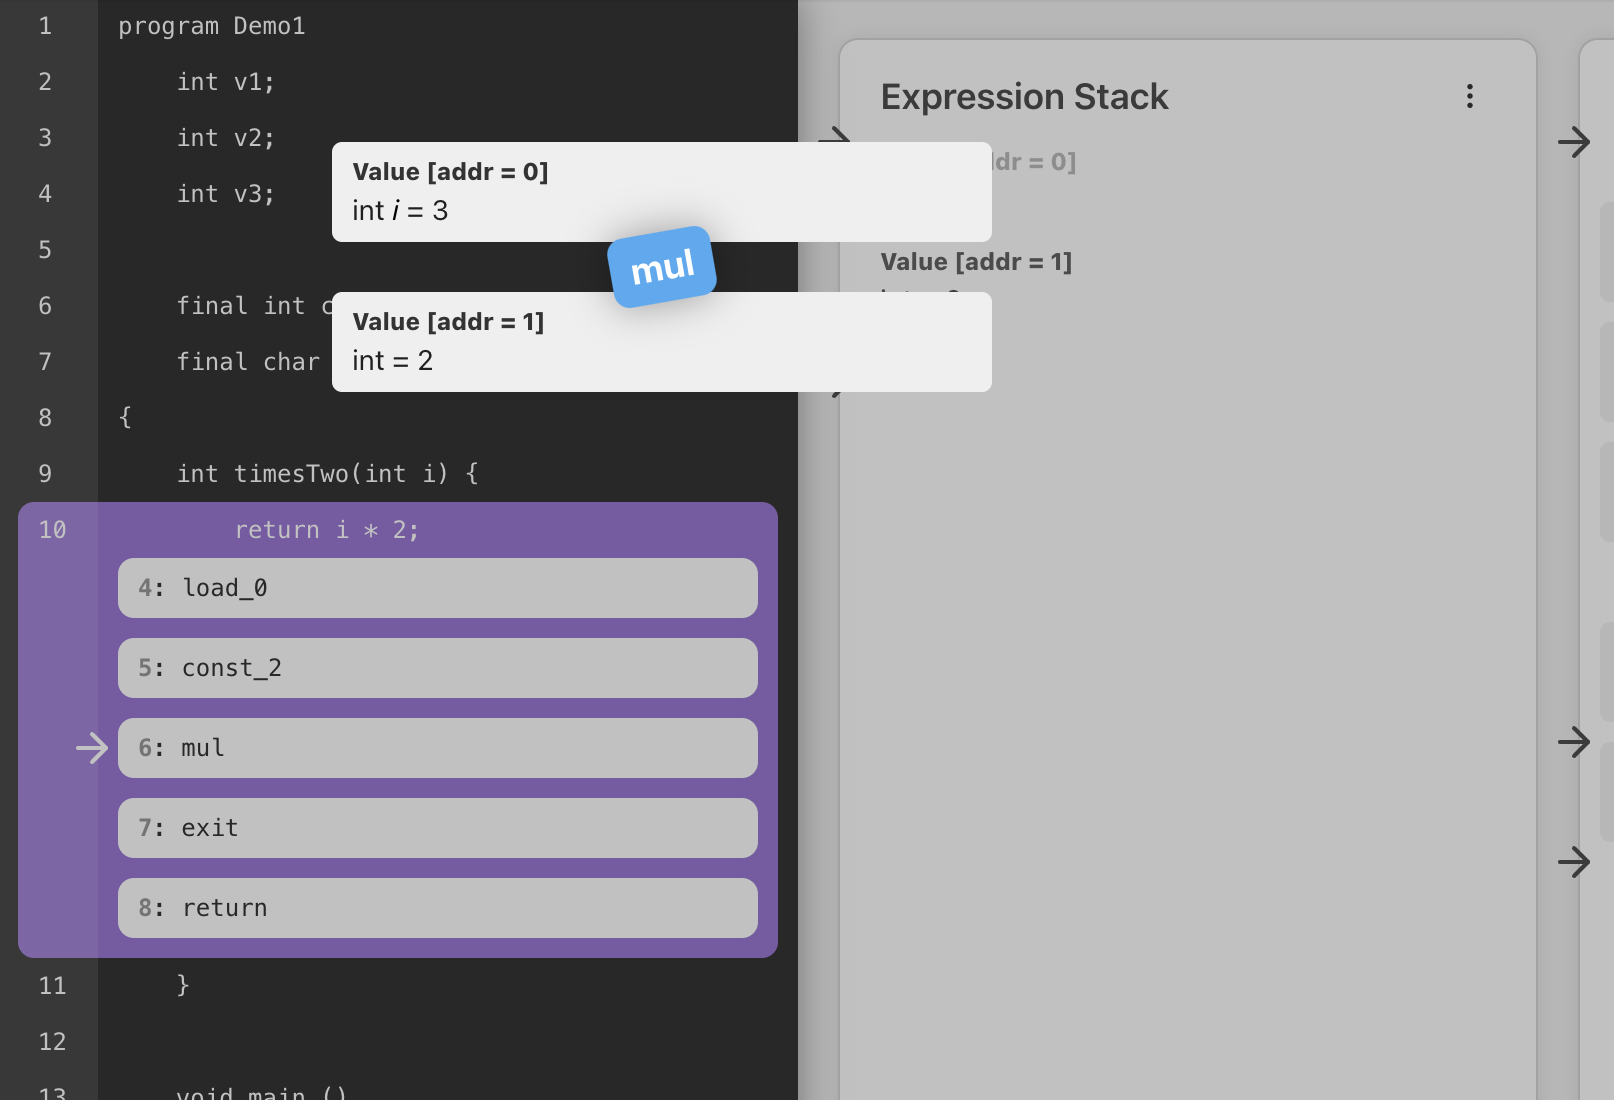
\includegraphics[width=0.5\textwidth]{fig/demo_arith1_1}
\caption{\label{fig:arith1} An in-progress multiplication operation animation symbolizing how two input memory entries are merged together to produce a single output memory entry.}
\end{figure}

\subsection{Heap Allocation (see \cite{herber2025}, Section VI-B)}

The \emph{Heap Allocation} demo builds on the previous example by introducing dynamic memory management. The program performs object and array allocations, populating the heap with structured data.

As detailed in~\cite{herber2025}, Section VI-B, reference memory entries are visualized with dashed borders. When hovering over a reference entry, the visualization highlights the referenced memory region, making pointer relationships more intuitive.

Additionally, the memory entries that make up memory structures, such as arrays and objects, are grouped together with enclosing boxes and type labels (see \cite{herber2025}, Section VI-D), as depicted in \autoref{fig:heap1}. Instead of presenting the memory entries individually, this allows users to visually associate memory entries with their underlying structures.

\begin{figure}[h]
\centering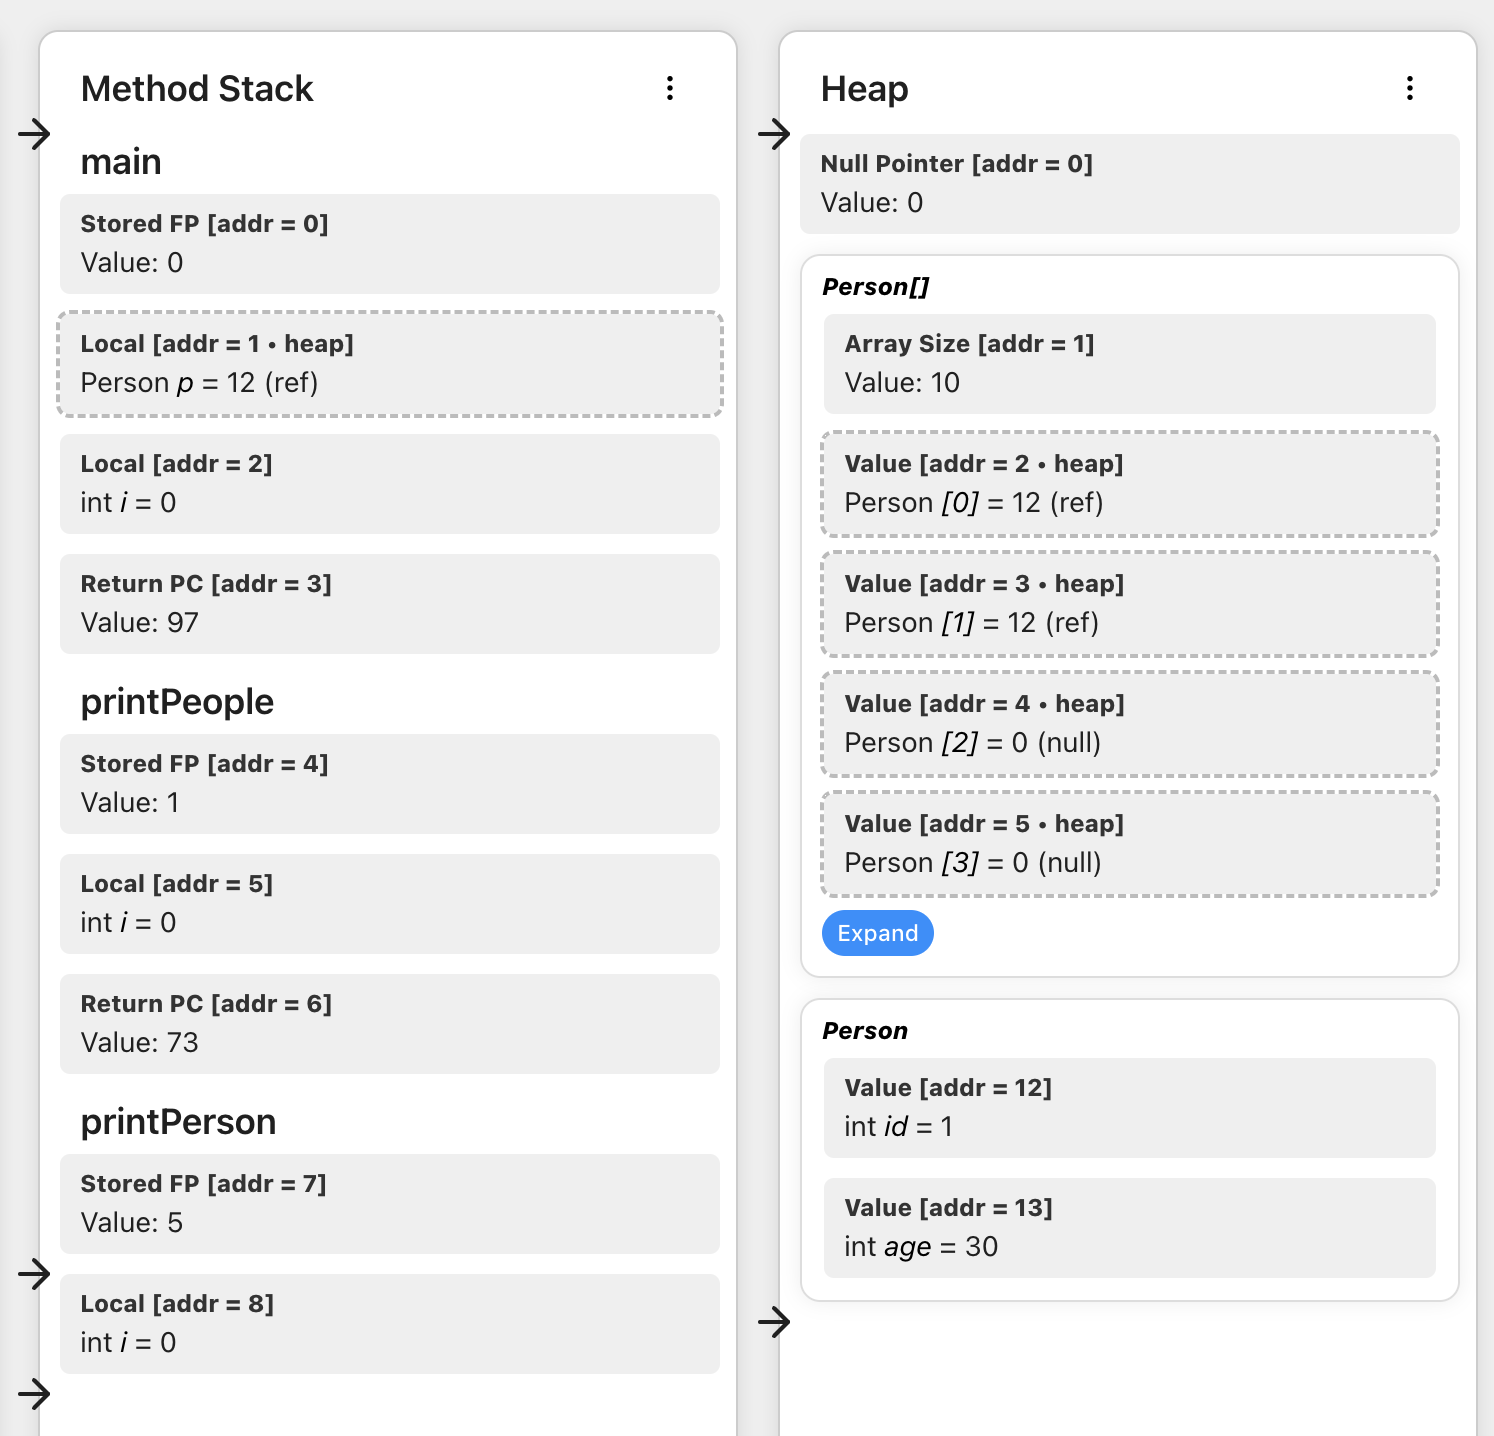
\includegraphics[width=0.45\textwidth]{fig/demo_heap1_1}
\caption{\label{fig:heap1} The method stack and heap regions. The heap region contains a \texttt{Person} array as well as a \texttt{Person} object.}
\end{figure}

\subsection{Control Flow (see \cite{herber2025}, Section V-B)}

The \emph{Control Flow} demo contains a trace of a program which implements a complicated conditional statement using short-circuit evaluation. This highlights our tool's capability to visualize complex control flow behavior, as outlined in \cite{herber2025}, Section V-B.

Jump operations in the bytecode are visualized using arrows that connect source and destination instructions, as shown in \autoref{fig:control1}. All branches of the control structure (e.g., if, else, elseif) are marked collectively, making their relationship easily understandable.

This example is particularly useful for understanding how high-level control constructs are compiled into low-level jumps and how they are optimized using short-circuit evaluation.

\begin{figure}[h]
\centering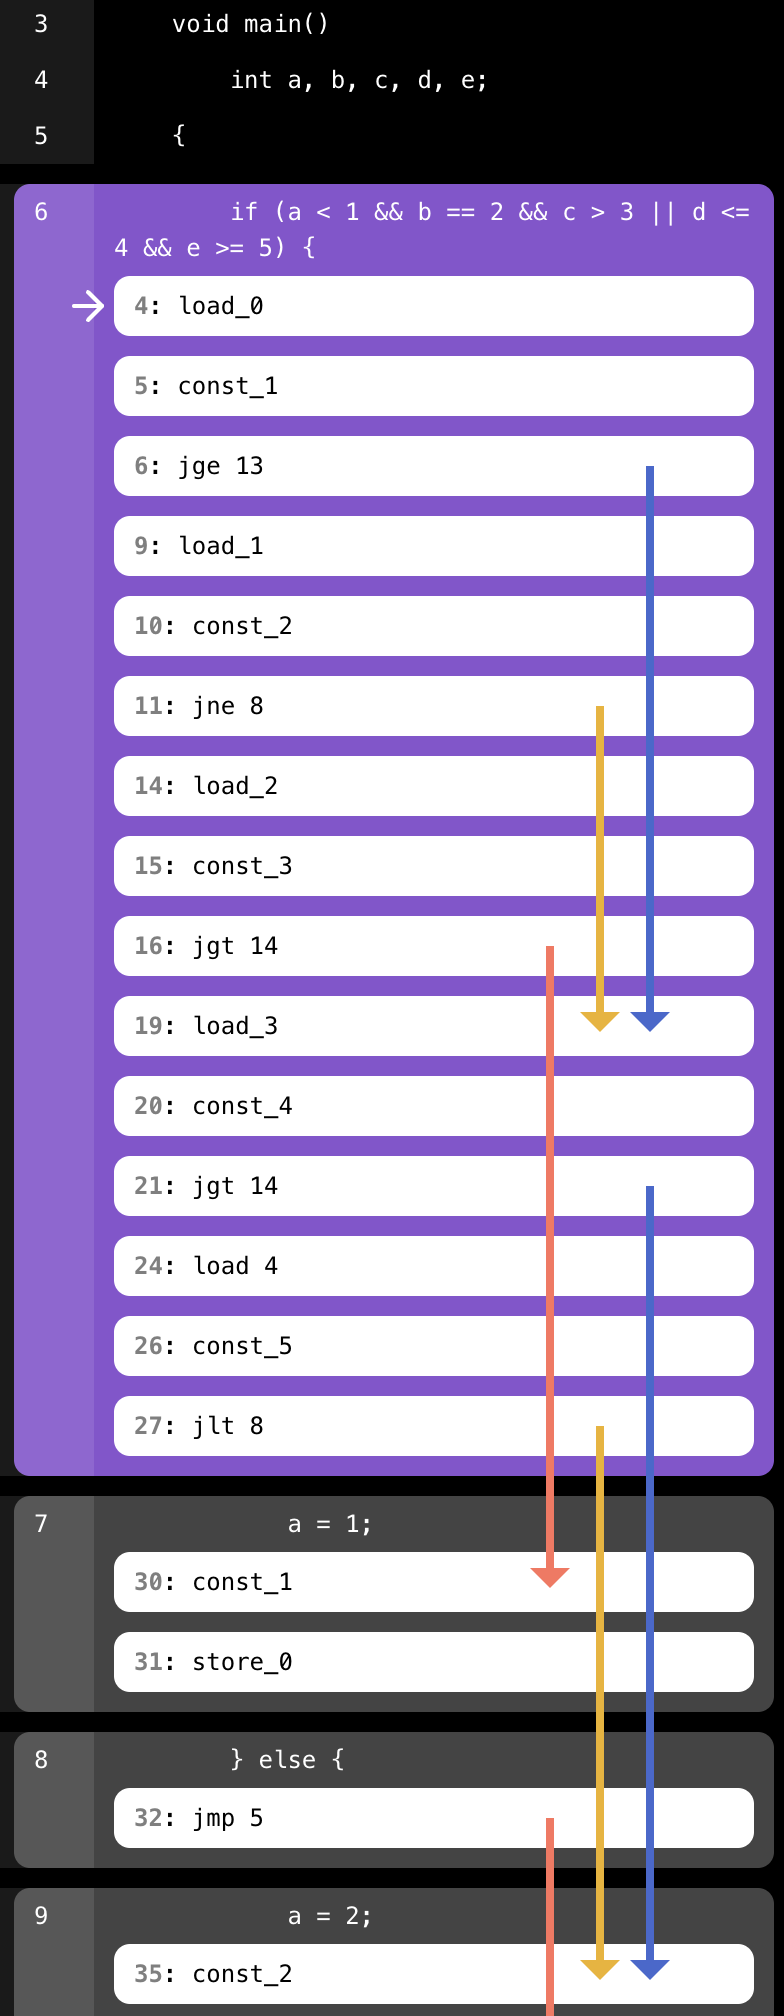
\includegraphics[width=0.35\textwidth]{fig/demo_control1_1}
\caption{\label{fig:control1} A complex if statement and the complex control flow operation used to implement it.\vspace{-1em}}
\end{figure}

\subsection{Interpreter Error (see \cite{herber2025}, Section IV-C)}

The \emph{Interpreter Error} demo show how our visualization handles faulty bytecode and bytecode interpreter failures. As described in \cite{herber2025}, Section IV-C, the trace includes error metadata that is presented in the visualization at the point of failure.

When stepping through this example, users will encounter an erroneous operation. Specifically, a stack underflow, where our compiler has generated two \texttt{ADD} operations instead of one, which means that the expression stack does not have the required two input memory entries for the second \texttt{ADD} operation. The visualization not only halts execution at this point, but also highlights the faulty instruction and its memory context, helping users find the root cause. Moreover, each error code has an associated hint which briefly describes what the error could mean, as depicted in \autoref{fig:int1}.

This feature is especially useful for students debugging their own compiler implementations, offering concrete visual feedback rather than abstract error messages. It should also be noted that bytecode errors are often more complex than a single invalid operation. Our visualization solves this by allowing users to step through the entire execution leading up to the error, thereby enabling concrete exploration of erroneous bytecode.

\begin{figure}[h!]
\centering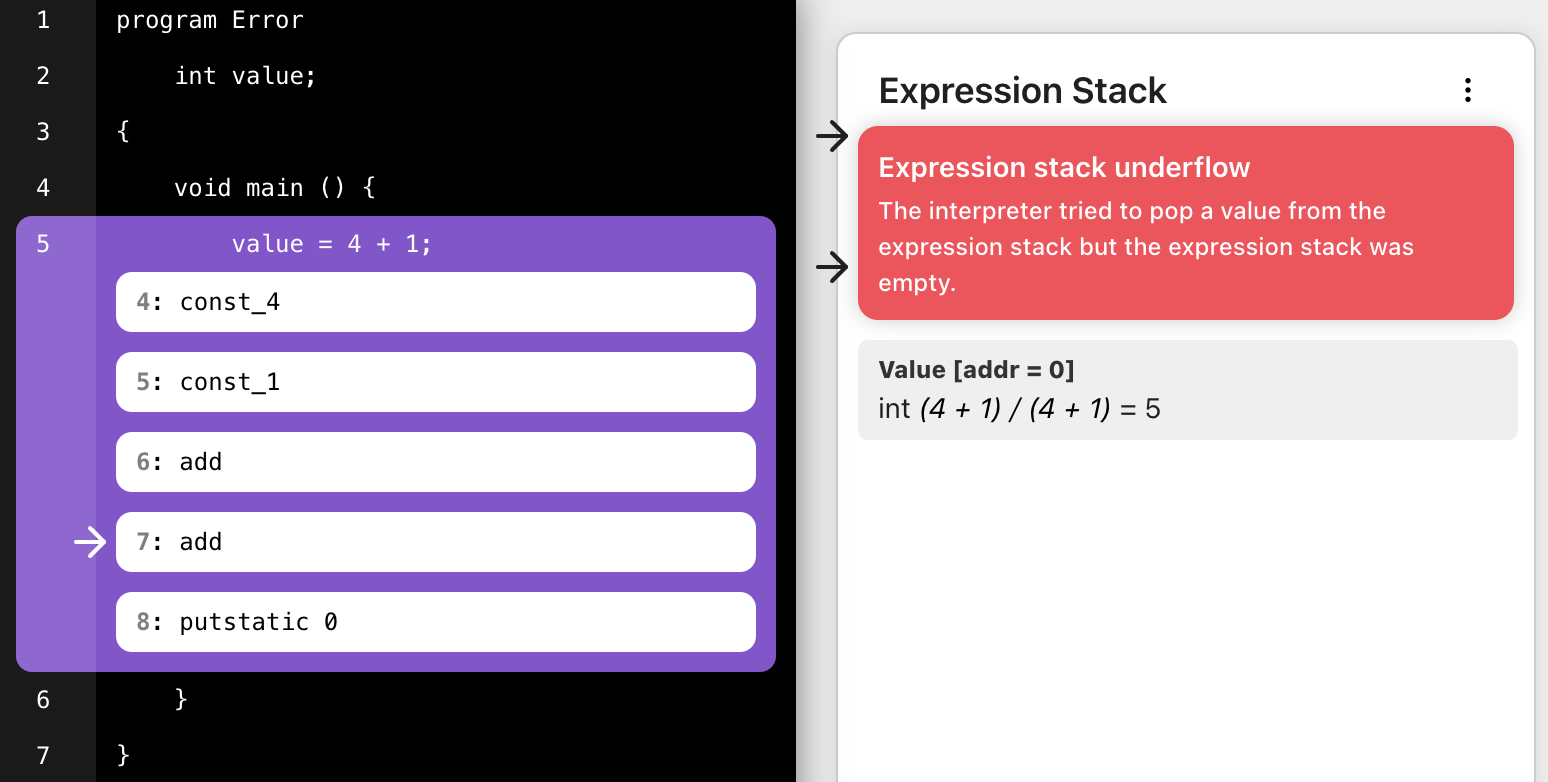
\includegraphics[width=0.5\textwidth]{fig/demo_ierr1_1}
\caption{\label{fig:int1} An erroneous bytecode operation and the corresponding interpreter error displayed in the expression stack memory region.\vspace{-1em}}
\end{figure}

\begin{figure}[h!]
\centering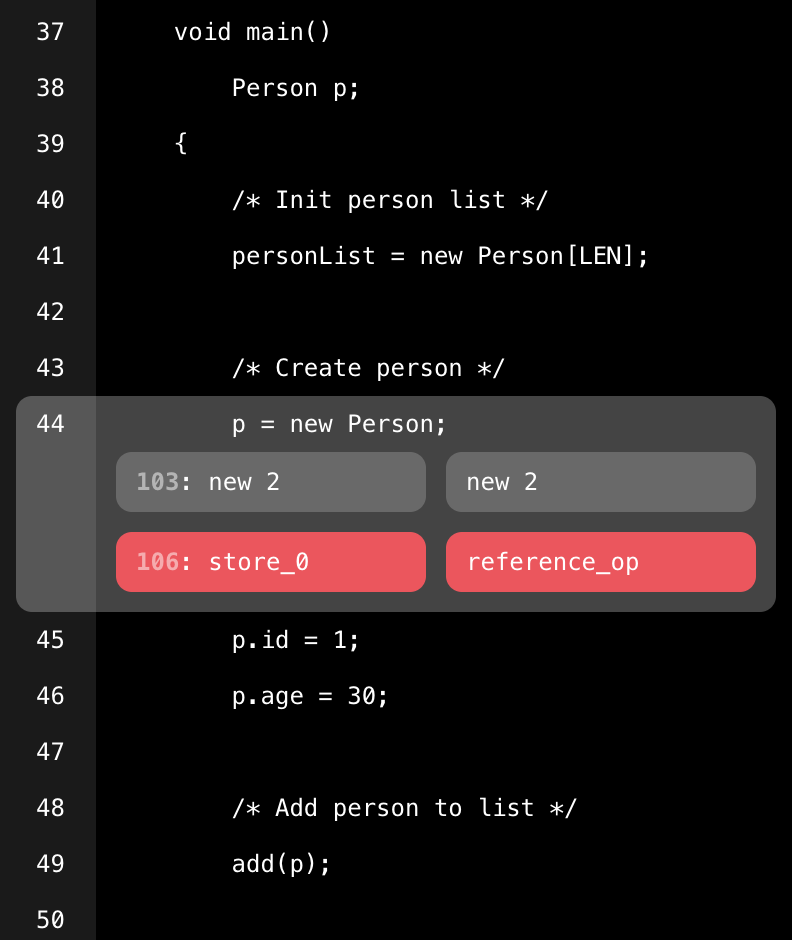
\includegraphics[width=0.5\textwidth]{fig/demo_ref1_1}
\caption{\label{fig:ref1} The code visualization where a single bytecode operation is highlighted because it does not match the reference bytecode.\vspace{-1em}}
\end{figure}

\subsection{Reference Bytecode (see \cite{herber2025}, Section V-C)}

Finally, the \emph{Reference Bytecode} demo illustrates our support for highlighting the discrepancy between expected and actual bytecode sequences. As detailed in \cite{herber2025}, Section V-C, this feature compares the student-generated bytecode against a reference implementation and highlights divergences directly within the user interface.

In this example, users see the actual and reference bytecode listed in parallel columns. Invalid instructions are colored red, and their origin is linked back to the source code using the bytecode-to-line mapping, as displayed in \autoref{fig:ref1}. This comparison enables students to immediately identify whether incorrect bytecode was generated.

These bytecode traces provide concrete examples of our visualization tool's core functionality. We encourage readers to try our hosted instance at \url{https://ssw.jku.at/General/Staff/Weninger/Projects/InterpreterViz/VISSOFT25/demo}.

\bibliographystyle{IEEEtran}
\bibliography{IEEEabrv, bibliography.bib}

\end{document}
